\section{Mergesort}

\textbf{Mergesort} ist ein \textbf{stabiler}, auf Schlüsselvergleichen basierender \textbf{interner} Sortieralgorithmus, der \textbf{nicht in place} sortiert.

\subsection{Methode}

\textbf{Mergesort} nutzt \textbf{divide-and-conquer}, um ein Feld zu sortieren.\\
Die wesentliche Arbeit erfolgt hier in den Merge-Schritten, im Gegensatz zu \textbf{Quciksort}, bei dem die eigentliche Arbeit im Partitionierungs-Schritt stattfindet (vgl.~\cite[174]{GD18e}).\\
I.d.R. wird bei Mergesort linear viel zusätzlichen Speicherplatz (vgl.~\cite[112]{OW17b}.

\noindent
Der Algorithmus teilt die Eingabefolge rekursiv in zwei gleich-große Folgen auf, bis $n$ ein-elementige Folgen vorhanden sind.\\
Im Anschluss werden die Folgen miteinander verschmolzen, und zwar so, dass die miteinander verschmolzenen Folgen immer in sortierter Reihenfolge vorliegen.\\
Das ganze wird so lange wiederholt, bis die Folge mit $n$ Elementen wieder komplett rekonstruiert ist (s. Abbildung~\ref{fig:mergesort}).

\subsection{Implementierung}

Das folgende Beispiel beinhaltet nicht die Methoden für die Partitionierung und das Verschmelzen.

\begin{minted}{java}
    mergeSort(int[] arr, int start, int end) {
        if (arr.length == 1) {
            return arr;
        }

        int mid = (start + end) / 2;
        int[] left = divide(arr, start, mid);
        int[] right = divide(arr, mid + 1, end);

        left = mergeSort(left, 0, left.length - 1);
        right = mergeSort(right, 0, right.length - 1);

        arr = merge(arr, left, right, start);

        return arr;
    }

\end{minted}

\begin{figure}
    \begin{center}
        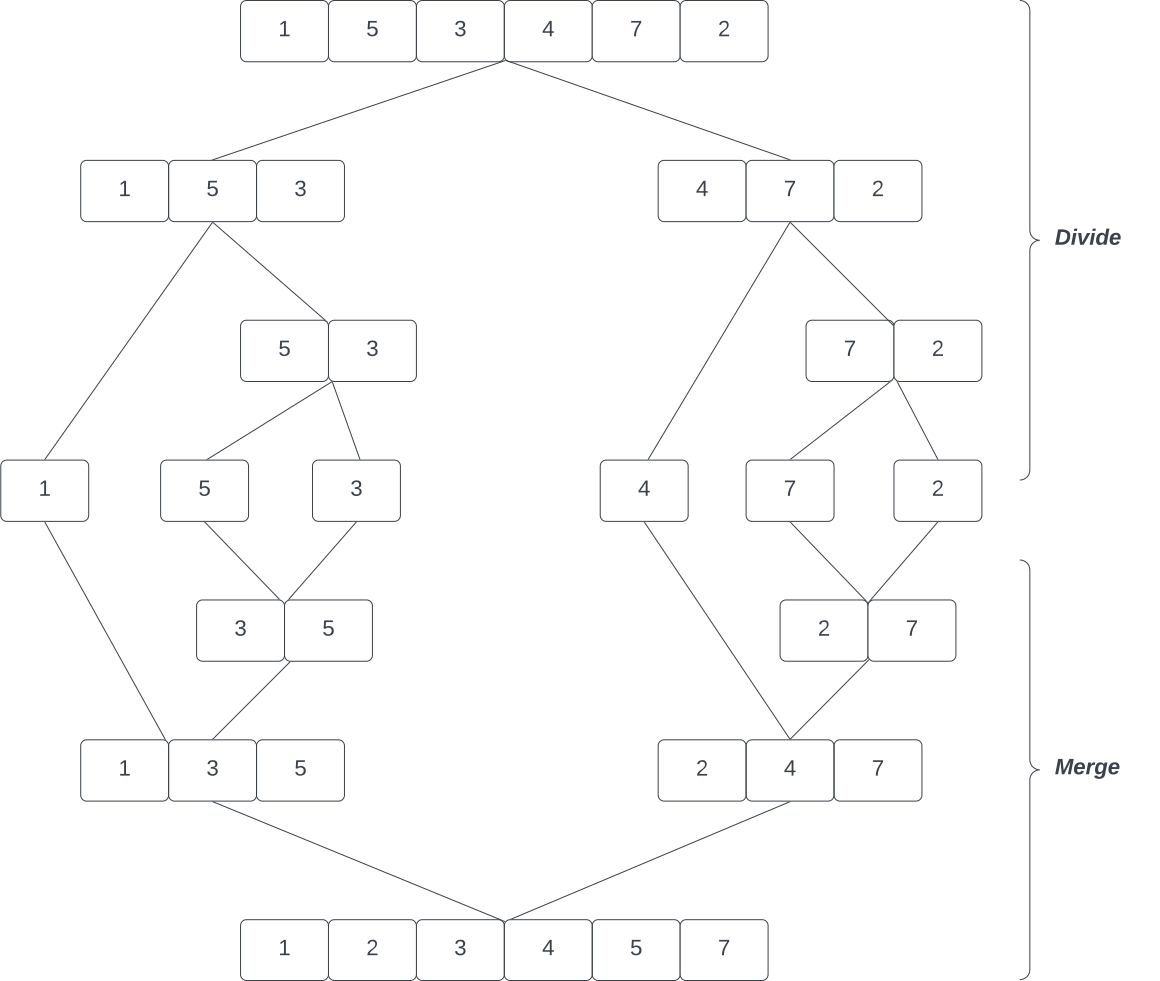
\includegraphics[scale=0.3]{chapters/Sortierverfahren/img/mergesort}
        \caption{Anwendung von Mergesort auf das Feld $1,\ 5,\ 3,\ 4,\ 7,\ 2$.  (Quelle: eigene)}
        \label{fig:mergesort}
    \end{center}
\end{figure}


\subsection{Laufzeit}
Im \textbf{worst-case} hat Mergesort eine Laufzeit von $O(n\ log\ n)$.